
\section{Introduction}

L'échantillonnage de pairs constitue le mécanisme fondamental de nombreuses
applications distribué à large échelle, que ce soit sur l'info-nuagique (REF) ou
en pair-à-pair. Les services de dissémination d'informations (REF),
d'aggrégation, de gestion de réseau sont basés sur l'échantillonnage de pairs et
la récente arrivée de WebRTC ouvre la possibilité de déployer de telles
applications dans les navigateurs, que ce soit sur portable, smartphone, etc. 
Dans ce contexte, WebRTC simplifie drastiquement le deploiement, même dans le
cadre de systèmes réseaux complèxes impliquant parefeu, proxies, et Net Address
Translation (NAT).

Malheureusement, WebRTC a de nombreuses containtes qui rendent les services
d'échantillonnage de pairs soit innéficaces, soit peu fiables. Sachant que les
navigateurs peuvent tourner sur de petit dispositifs aux ressources limitées,
conserver le nombre de connections aussi peu nombreuse que possible est un enjeu
majeur. Cependant, les services d'échantillonnage de pairs tels que \CYCLON
n'adapte pas leur nombre de connections aux nombres de pairs dans le réseau. Par
exemple, un utilisateurs peut maintenir 10 connexions actives avec des
navigateurs distants lorsque seulement 6 sont suffisantes. A l'opposé, le
protocole d'échantillonnage de pairs nommé \SCAMP est adaptatif. Toutefois, il
utilise dissémine systématiquement les connections aléatoirement dans le réseau
ce qui est beaucoup plus couteux et prompt à l'échec dans le contexte WebRTC.

Dans cette section, nous présentons \SPRAY, un protocole d'échantillonnage
aléatoire inspiré à la fois de \SCAMP et de \CYCLON. Comparé à l'état de l'art,
\begin{inparaenum}
\item \SPRAY adapte dynamiquement le voisinage de chaque pairs. Ainsi le nombre
  de connections augmente logarithmiquement par rapport à la taille du réseau.
\item \SPRAY n'utilise que des interactions de voisin à voisin pour établir les
  connections. Ainsi, celles-ci sont établies en temps constant.
\item \SPRAY converge rapidement vers une topologie possédant des propriétés
  similaires à celles des graphes aléatoires. Ainsi, le réseau est robuste aux
  défaillances massives, dissémine les informations de manière efficiace, etc.
\end{inparaenum}
Les expériences montre l'adaptivité de \SPRAY et mette en évidence ses
améliorations face à \CYCLON et \SCAMP, à un prix minime.
  



\subsection{Champs d'applications}

\subsubsection{Dissémination d'informations}
\subsubsection{Gestion de topologies réseau}

\subsection{WebRTC}

\begin{figure*}
\centering
\subfloat[Figure A][\label{fig:webrtcA}
$p_1$ connects to $p_2$ using the signaling service.
1: $p_1$ pushes its offer ticket;
2: $p_2$ pulls the ticket;
3: $p_2$ pushes its response;
4: $p_1$: pulls the response and establishes a
bidirectional connection with $p_2$. $p_3$ does the same with $p_2$.
Figure~\ref{fig:webrtcB} depicts the resulting network.]{
  
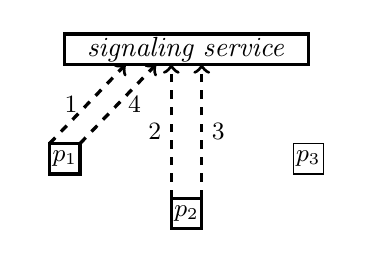
\begin{tikzpicture}[scale=1.1]

\newcommand\X{40pt};
\newcommand\Y{18pt};

\draw( 1.3*\X, 0); %% spacing
\draw(-1.3*\X, 0); %% spacing

\draw[fill=white,very thick](0*\X, 0*\Y) 
node{\emph{signaling service}} +(-40pt,-5pt) rectangle +(40pt,5pt);

\small
\draw[->,dashed, very thick](-5 -1*\X, 5-2*\Y) --
node[anchor=east]{1} (-20pt,-5pt);
\draw[->,dashed, very thick]( 5 -1*\X, 5-2*\Y) --
node[anchor=west]{4} (-10pt,-5pt);

\draw[->,dashed, very thick](-5pt,  5-3*\Y) --
node[anchor=east]{2}(-5pt,-5pt);
\draw[->,dashed, very thick](5pt , 5-3*\Y) --
node[anchor=west]{3} (5pt,-5pt);


\draw[fill=white, very thick]
(-1*\X,-2*\Y) node{$p_1$} +(-5pt,-5pt) rectangle +(5pt,5pt);
\draw[fill=white, very thick]
(0*\X, -3*\Y) node{$p_2$} +(-5pt,-5pt) rectangle +(5pt,5pt);
\draw[fill=white] (1*\X, -2*\Y) node{$p_3$} +(-5pt,-5pt) rectangle +(5pt,5pt);

\end{tikzpicture}

% \begin{tikzpicture}
% \matrix (m) [matrix of math nodes,row sep=4em,column sep=4em] {
% \node(ss)[draw]{signaling}; & \node(p3)[draw]{p3}; \\
% \node(p1)[draw]{p1}; & \node(p2)[draw]{p2}; \\
% };
% \path[->]
%   (p2) edge[dashed] node[fill=white]{1:emit} (ss)
%   (p3) edge[dashed] node[fill=white,bend left]{2:pull} (ss)
%   (p3) edge[dashed, bend right] node[fill=white]{3:accept} (ss)
%   (p2) edge[dashed,bend left] node[fill=white]{4:pull} (ss)
%   (p3) edge[<->,thick] node[fill=white,right]{5:connected} (p2);
% \end{tikzpicture}}
\hspace{5pt}
\subfloat[Figure B][\label{fig:webrtcB}
$p_1$ connects to $p_3$ using $p_2$ as mediator.
1: $p_1$ sends its offer ticket to $p_2$;
2: $p_2$ forwards it to $p_3$ and registers $p_1$ as the emitter;
3: $p_3$ sends its response to $p_2$;
4: $p_2$ forwards it to the emitter $p_1$ which connects to $p_3$.]{
  
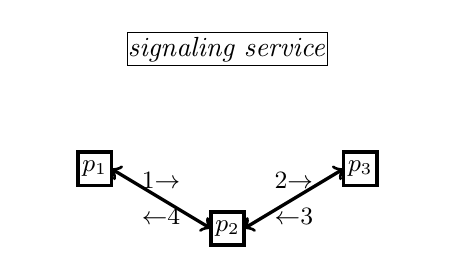
\begin{tikzpicture}[scale=1.2]

\newcommand\X{40pt};
\newcommand\Y{18pt};

\draw(1.5*\X, 0); %% spacing
\draw(-1.5*\X, 0); %% spacing

\draw[fill=white](0*\X, 0*\Y)
node{\emph{signaling service}} +(-30pt,-5pt) rectangle +(30pt,5pt);

\small
\draw[<->, very thick](5-1*\X,-2*\Y)--
node[anchor=south]{1$\rightarrow$}
node[anchor=north]{$\leftarrow$4}(-5pt,-3*\Y);
\draw[<->, very thick](5pt,-3*\Y)--
node[anchor=south]{2$\rightarrow$}
node[anchor=north]{$\leftarrow$3}(-5+1*\X,-2*\Y);

\draw[fill=white, very thick]
(-1*\X,-2*\Y) node{$p_1$} +(-5pt,-5pt) rectangle +(5pt,5pt);
\draw[fill=white, very thick]
(0*\X, -3*\Y) node{$p_2$} +(-5pt,-5pt) rectangle +(5pt,5pt);
\draw[fill=white, very thick]
(1*\X, -2*\Y) node{$p_3$} +(-5pt,-5pt) rectangle +(5pt,5pt);

\end{tikzpicture}

% \begin{tikzpicture}
% \matrix (m) [matrix of math nodes,row sep=4em,column sep=4em] {
% \node(ss)[draw]{signaling}; & \node(p3)[draw]{p3}; \\
% \node(p1)[draw]{p1}; & \node(p2)[draw]{p2}; \\
% };
% \path[->]
%   (p1) edge[dashed,bend left] node[fill=white]{1:emit} (p2)
%   (p2) edge[dashed,bend left] node[fill=white,left]{2:emit/p1} (p3)
%   (p3) edge[dashed,bend left] node[fill=white,right]{3:accept/p1} (p2)
%   (p2) edge[dashed,bend left] node[fill=white]{4:accept} (p1)
%   (p1) edge[<->,thick] (p2)
% %  (p1) edge[<->,thick,bend left] (p3)
%   (p2) edge[<->,thick]  (p3);

% \end{tikzpicture}}
\hspace{5pt}
\subfloat[Figure C][\label{fig:webrtcC}
The resulting network overlay: a fully connected network composed of
3 members.]{
  
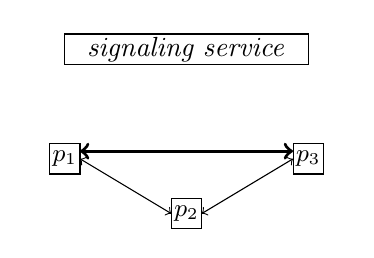
\begin{tikzpicture}[scale=1.1]

\newcommand\X{40pt};
\newcommand\Y{18pt};

\draw(1.3*\X, 0); %% spacing
\draw(-1.3*\X, 0); %% spacing

\draw[fill=white](0*\X, 0*\Y)
node{\emph{signaling service}} +(-40pt,-5pt) rectangle +(40pt,5pt);

\small
\draw[<->](5-1*\X,-2*\Y)--(-5pt,-3*\Y);
\draw[<->](5pt,-3*\Y)--(-5+1*\X,-2*\Y);
\draw[<->, very thick](5 - 1*\X, 2.5 -2*\Y)--(-5+1*\X, 2.5 -2*\Y);

\draw[fill=white]
(-1*\X,-2*\Y) node{$p_1$} +(-5pt,-5pt) rectangle +(5pt,5pt);
\draw[fill=white]
(0*\X, -3*\Y) node{$p_2$} +(-5pt,-5pt) rectangle +(5pt,5pt);
\draw[fill=white]
(1*\X, -2*\Y) node{$p_3$} +(-5pt,-5pt) rectangle +(5pt,5pt);

\end{tikzpicture}


% \begin{tikzpicture}
% \matrix (m) [matrix of math nodes,row sep=4em,column sep=4em] {
% \node(ss)[draw]{signaling}; & \node(p3)[draw]{p3}; \\
% \node(p1)[draw]{p1}; & \node(p2)[draw]{p2}; \\
% };
% \path[->]
%   (p1) edge[<->,thick] (p2)
%   (p1) edge[<->,thick] (p3)
%   (p2) edge[<->,thick]  (p3);
% \end{tikzpicture}}
\caption{\label{fig:webrtc}Creating an overlay network on top of WebRTC.}
\end{figure*}


WebRTC permet la communication en temps réel entre navigateurs web et ce, même
en présence de configurations réseaux complexes impliquant firewall, proxy, ou
NAT (Network Address Translation). Toutefois, WebRTC ne gère ni l'adressage, ni
le routage. Pour établir une connexion, les navigateurs s'échangent des offres
et acquittements via un médiateur commun (e.g. mails, services dédiés de
signalement, connections WebRTC connues, etc.). Dans la
figure~\ref{fig:webrtcA}, $p_1$ souhaite se connecter à $p_2$. Par conséquence,
$p_1$ envoie son ticket d'offre au service de signalement connu. Le pair $p_2$
récupère l'offre, la poinçonne et la renvoie au service de signalement. Enfin,
$p_1$ récupère le ticket poinçonné et établie une connexion bidirectionnelle
avec $p_2$. De manière identique, $p_3$ établie une connexion avec $p_2$. Nous
appellerons la procédure d'aller-retour des tickets un \emph{three-way
  handshake}. Désormais, le pair $p_1$ est capable d'établir une connexion avec
$p_3$ sans passer par l'intermédiaire du serveur. Pour cela, il utilise $p_2$
comme médiateur. Toutefois, si le pair $p_2$ crash durant cette procédure, la
connexion ne pourra s'effectuer correctement, et ce même si une route
alternative existe (puisque WebRTC ne gère pas le routage).

Utiliser les services de signalement et les connections WebRTC existantes permet
de déployer facilement les protocoles d'échantillonnage aléatoire de
pairs~\cite{jelasity2007gossip}. Ces derniers étant présent dans les navigateurs
modernes disponibles sur les smartphones, les tablettes, etc. Dans ce contexte,
il est impératif de conserver autant que possible un petit nombre de connections
afin de réduire le trafic réseau et limiter la consommation de ressources.


\subsubsection{Facilité d'accès}
\subsubsection{Contraintes supplémentaires}


%%% Local Variables:
%%% mode: latex
%%% TeX-master: "../../paper"
%%% End:
